\documentclass[12pt]{article}

\usepackage[a4paper, total={6in, 9in}]{geometry}
\usepackage[hidelinks]{hyperref}
\hypersetup{
    colorlinks=true,
    linkcolor=blue,    
    urlcolor=cyan,
    pdfborder={0 0 0},       % Disables the border around links
    linkbordercolor={0 0 0}, % Disables yellow hover highlighting
}
\usepackage[english, activeacute]{babel}
\usepackage[utf8]{inputenc}
\usepackage[T1]{fontenc}
\usepackage{amsmath}
\usepackage{graphicx}
\usepackage{float}
\usepackage{amsthm}
\usepackage{amsfonts}
\usepackage{bookmark}
\usepackage{enumitem}
\usepackage[parfill]{parskip}
\usepackage{minted} 
\usepackage{multicol}
\usepackage{caption}
\usepackage{graphicx} % Package to insert images
\graphicspath{ {images/} } % Path to images directory

\title{Preliminary Report}
\author{Diego Chiola, Alex Valle, Gabriele Berruti}
\date{10/01/2025}

\begin{document}
\maketitle
\newpage

\section{Topic}
The main topic of our final project will be about digitalization in the European
Union countries, more precisely we want to analyze three aspects:
\begin{enumerate}
    \item \textbf{The level of access to the internet}: how many have access to the
          internet, with which devices and how this percentage has changed over time.
    \item \textbf{Internet uses}: how often people use the internet, for what purposes,
          negative experiences of users, to then do a more in-depth analysis for some
          sectors such as e-commerce and financial activities.
    \item \textbf{Digital skills}: the skills that people have in using the internet,
          the number of people who have ICT education divided by sex, age and educational
          attainment level.
\end{enumerate}

\section{Datasets}
Digitalization
\href{https://ec.europa.eu/eurostat/web/digital-economy-and-society/database}{datasets}
\begin{itemize}
    \item Internet access section:
          \begin{itemize}
              \item Households - level of internet access
              \item Households - type of connection to the internet
              \item Households - devices to access the internet
              \item Households - reasons for not having internet access at home
          \end{itemize}

    \item Frequency and use type of internet:
          \begin{itemize}
              \item Individuals - frequency of internet use
              \item Individuals - internet activities
              \item Individuals - encountering hostile or degrading online messages
              \item Internet purchases by individuals
              \item Financial activities over the internet
          \end{itemize}
    \item Digital skill
          \begin{itemize}
              \item Individuals' level of digital skills
              \item ICT specialist in employment (by sex, age and educational attainment level)
          \end{itemize}
\end{itemize}

\section{Charts type}
In detail these are the graphs that we would like to use divided by topic:
\begin{enumerate}
    \item \textbf{Internet Access Level}
          \begin{itemize}
              \item Two views: a bar chart and a map for people who have access to the internet.
              \item A line chart showing the change over time for people who have never used the internet.
              \item A stacked bar chart with the types of devices used.
              \item An area chart to show how the reasons on why people do not have access to the internet changes over time.
          \end{itemize}
    \item \textbf{Uses of the Internet}
          \begin{itemize}
              \item A line chart showing how the percentage of individuals using the internet daily or at least once a
                    week varies over time.
              \item An alluvial/stacked bar chart depicting how people use the internet.
              \item Faceted bar chart for Data on individuals encountering hostile or degrading messages online,
                    focus on age groups (data of 2023).
              \item Grouped bar chart to show how the percentage of people who have made online purchases changes
                    over the year for different age group, with filtering options based on the last purchase date.
              \item Line/Bubble chart to show how Financial activities over the internet increase over the years divided by education level.
          \end{itemize}
    \item \textbf{Digital Skills}
          \begin{itemize}
              \item Two views: a bar chart to compare Individuals' level of digital skills between countries and a line chart to
                    see how this percentage change over the time.
              \item Stacked bar chart to show the percentage of males and females employed with ICT education (A line/area chart
                    can be added to show how this percentage varies over time).
              \item Stacked bar chart to show the percentage of individuals employed with ICT education that are between two age
                    group (A line/area chart can be added to show how this percentage varies over time).
              \item Alluvial chart to see how the employed persons with ICT education are distributed by educational attainment level.
          \end{itemize}
\end{enumerate}
\newpage

\subsection*{Bar chart}
\begin{figure}[h]
    \centering
    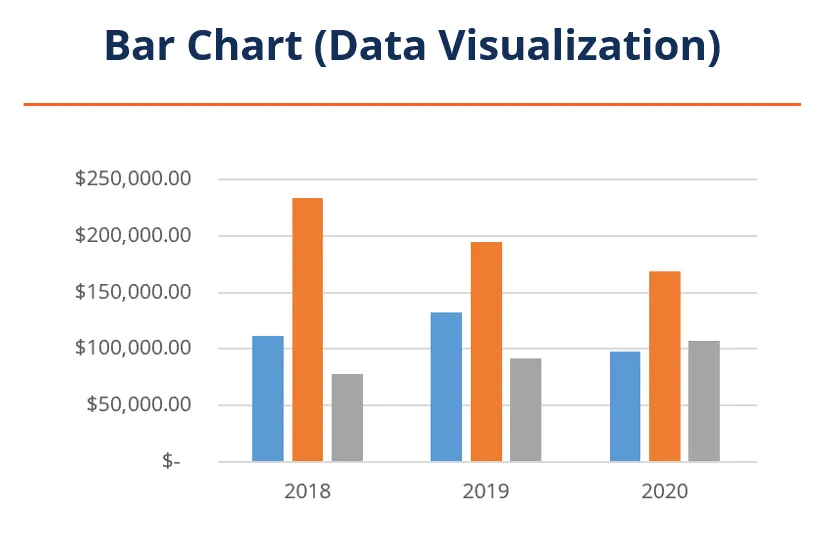
\includegraphics[width=12cm, height=8cm]{bar-charts.png}
    \centering
\end{figure}

\subsection*{Stacked Bar Chart}
\begin{figure}[h]
    \centering
    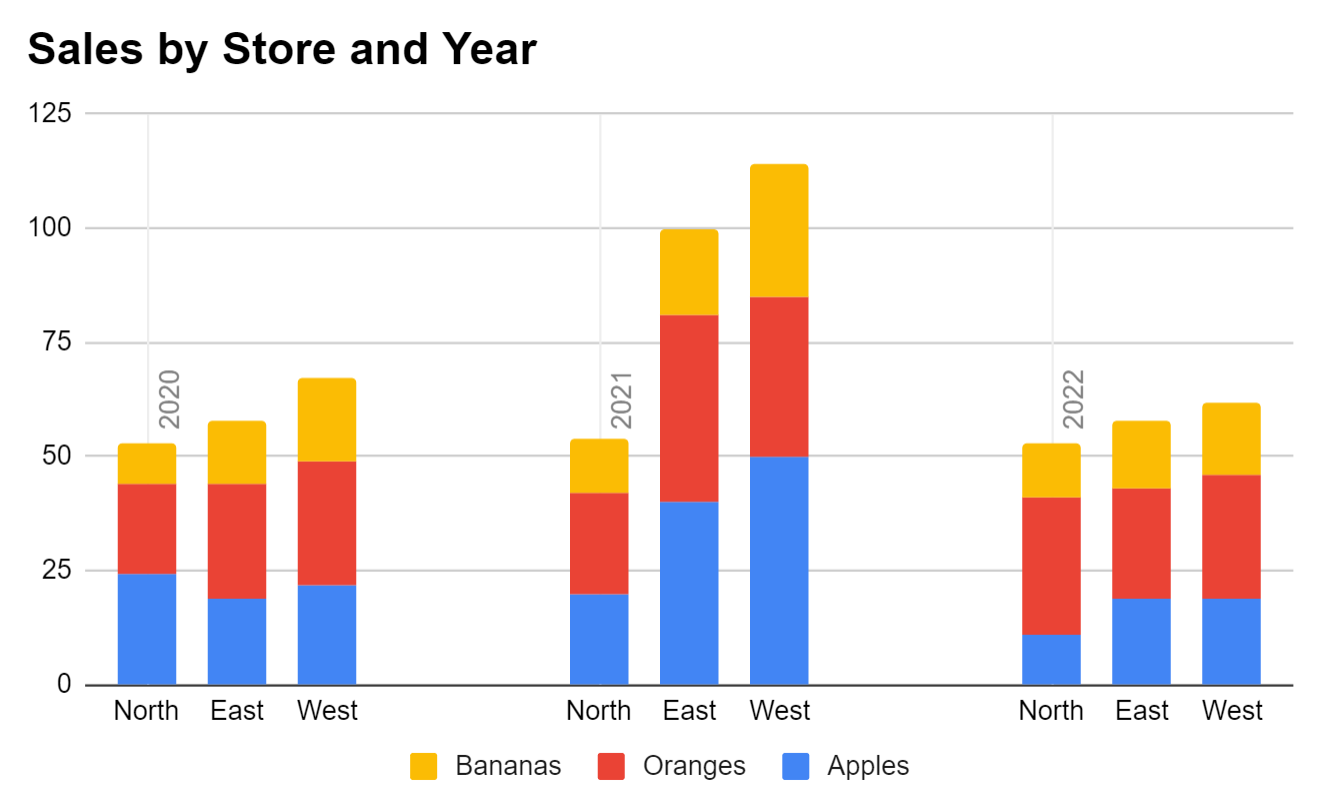
\includegraphics[width=12cm, height=8cm]{clusterstack1.png}
    \centering
\end{figure}

\newpage

\subsection*{Faceted Bar Chart}
\begin{figure}[h]
    \centering
    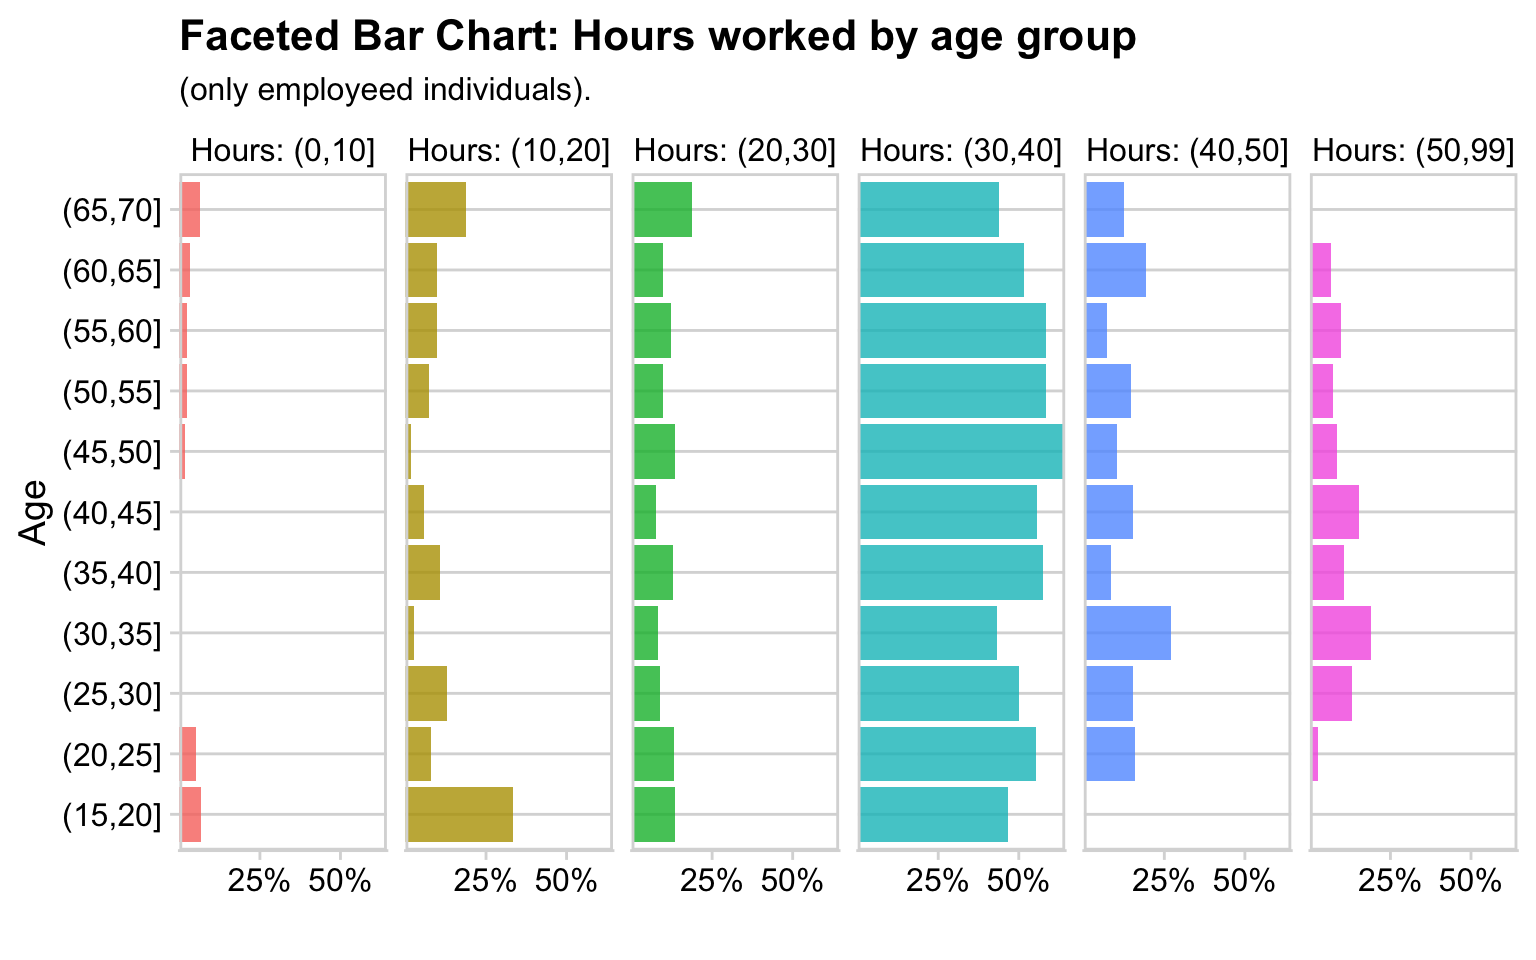
\includegraphics[width=12cm, height=8cm]{faceted-barchart.png}
    \centering
\end{figure}

\subsection*{Alluvial Chart}
\begin{figure}[h]
    \centering
    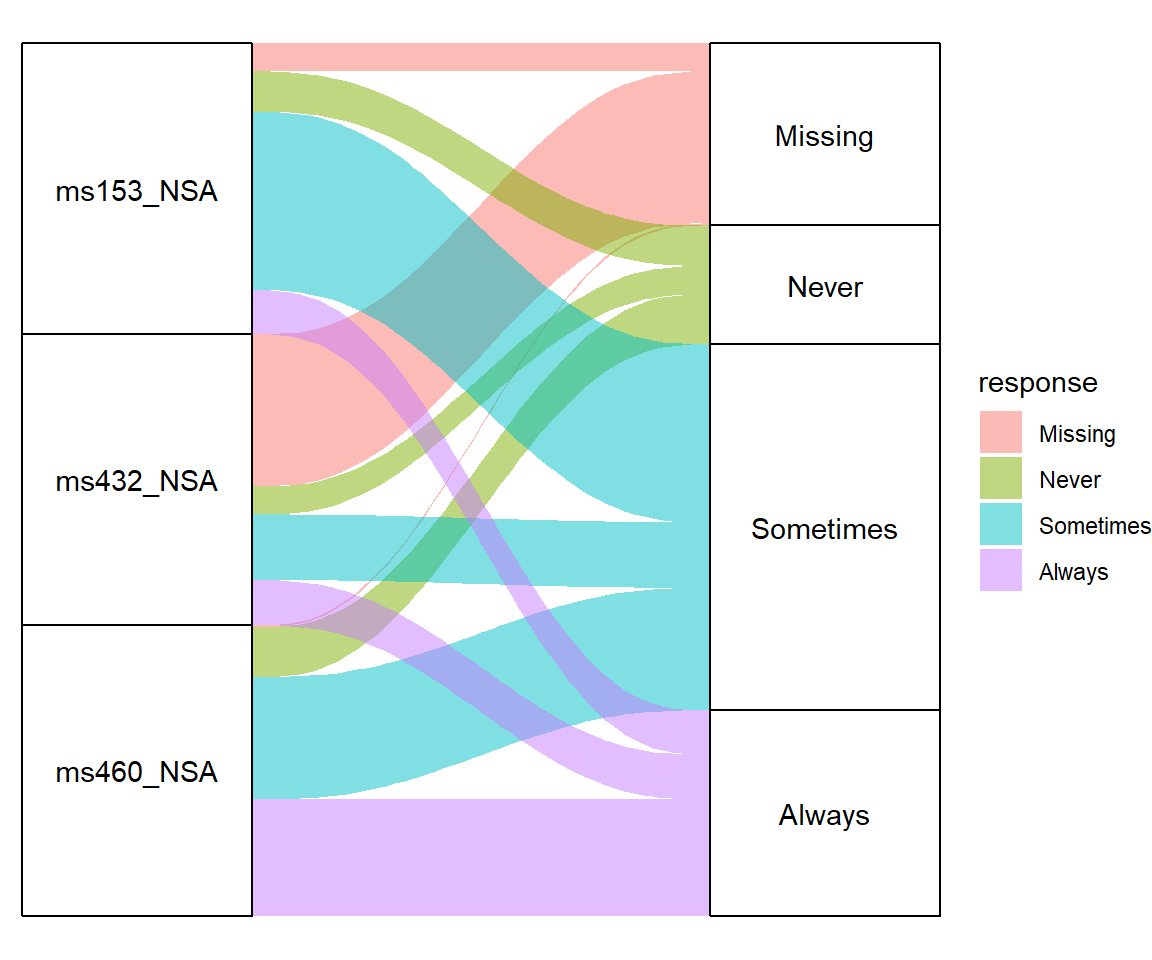
\includegraphics[width=12cm, height=8cm]{alluvial-plot-quintic.png}
    \centering
\end{figure}

\newpage

\subsection*{Map}
\begin{figure}[h]
    \centering
    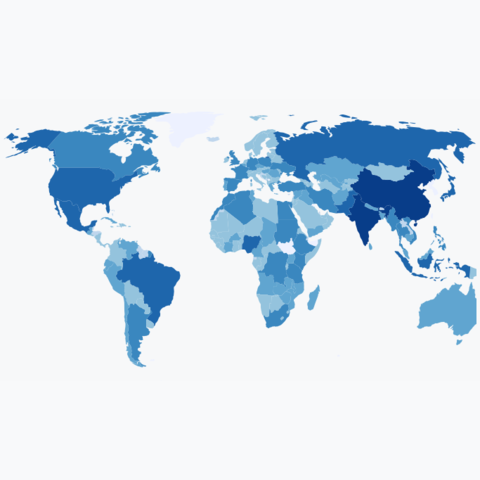
\includegraphics[width=12cm, height=8cm]{choropleth_basic.png}
    \centering
\end{figure}

\subsection*{Line Chart}
\begin{figure}[h]
    \centering
    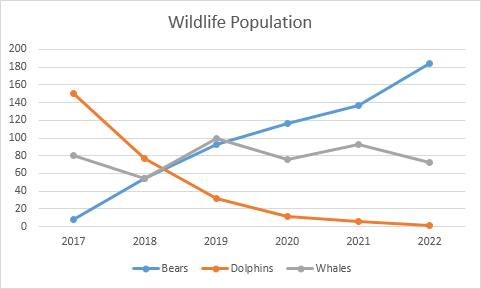
\includegraphics[width=12cm, height=8cm]{line-chart.png}
    \centering
\end{figure}

\newpage

\subsection*{Bubble Chart}
\begin{figure}[h]
    \centering
    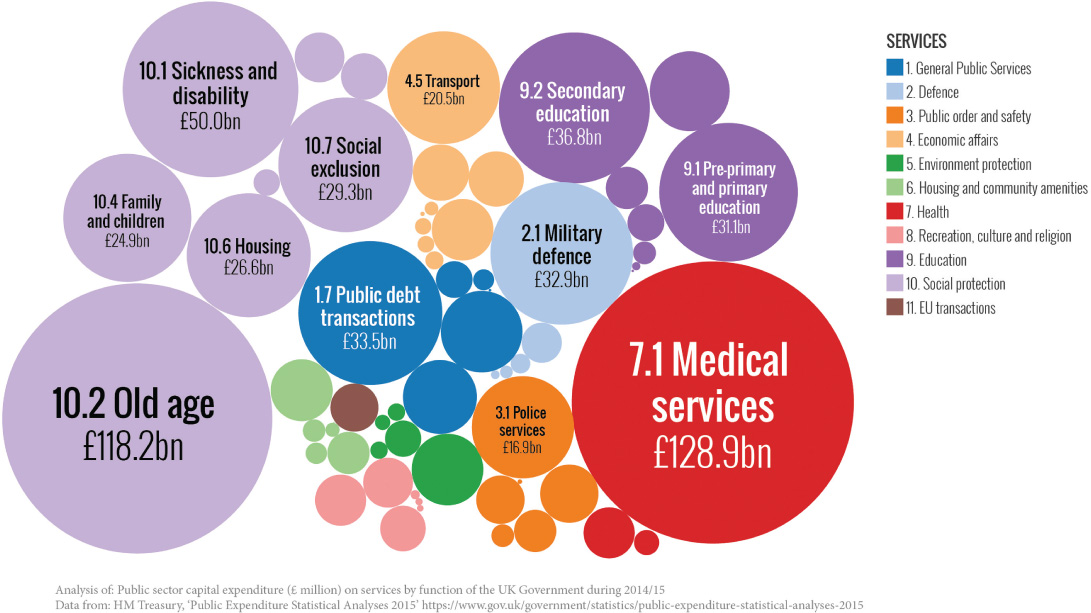
\includegraphics[width=13cm, height=8cm]{bubble-chart.png}
    \centering
\end{figure}

\subsection*{Area Chart}
\begin{figure}[h]
    \centering
    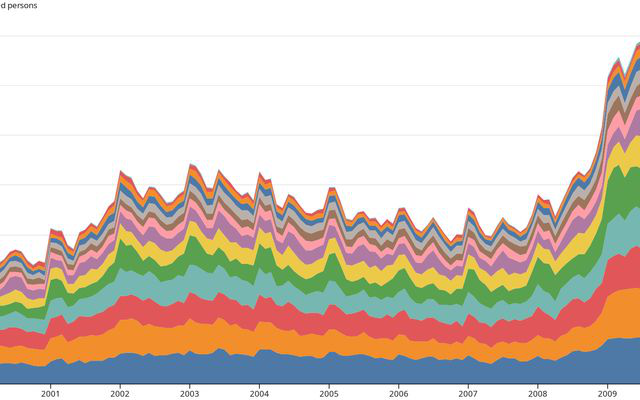
\includegraphics[width=13cm, height=8cm]{area-chart.png}
    \centering
\end{figure}


\end{document}